\documentclass[a4paper,14pt]{extarticle}
\usepackage[english,russian]{babel}
\usepackage[cache=false]{minted}
\usepackage{fontspec}
\usepackage{indentfirst}
\usepackage{listings}
\usepackage{color}
\usepackage{caption}
\usepackage{amsmath}
\usepackage{hyperref}
\usepackage{graphicx}
\usepackage[%
    left=20mm,%
    right=10mm,%
    top=20mm,%
    bottom=20mm,%
]{geometry}%
\usepackage{titlesec}


\setmainfont{PT Astra Serif}

\hypersetup{
    colorlinks=true,
    linkcolor=black,
    filecolor=magenta,
    urlcolor=cyan,
    pdftitle={Лабораторная работа №4},
    pdfpagemode=FullScreen,
}

\newcommand{\hlink}[2]{\href{#1}{\color{blue}\underline{#2}}}
\graphicspath{ {./images/} }

\setmonofont[Scale=0.8]{JetBrains Mono}
\setminted{frame=lines, framesep=3mm, fontsize=\small}
\usemintedstyle{vs}

\titleformat{\section}
{\normalfont\bfseries}{}{0pt}{Упражнение \thesection.\;}

\titleformat{\subsection}
{\normalfont\bfseries}{}{0pt}{Задание \thesubsection.\;}

\numberwithin{figure}{section}

\begin{document}

\begin{titlepage}
    \vspace{0pt plus2fill}
    \noindent

    \vspace{0pt plus6fill}
    \begin{center}
        \textbf{\large{Санкт-Петербургский национальный исследовательский университет информационных
                технологий, механики и оптики}}

        \vspace{0pt plus2fill}
        \textbf{\Large{ЛАБОРАТОРНАЯ РАБОТА №3}}

        \vspace{0pt plus2fill}
        \textbf{\large{Использование выражений}}
    \end{center}

    \vspace{0pt plus8fill}
    \begin{flushright}
        Студент: \\
        \textit{Швалов Даниил Андреевич}

        \textit{Факультет ИКТ}

        Группа: \textit{К32211}

        Преподаватель: \\
        \textit{Иванов Сергей Евгеньевич}
    \end{flushright}

    \vspace{0pt plus4fill}
    \begin{center}
        {Санкт-Петербург~--- 2023}
    \end{center}
\end{titlepage}

\section{Реализация операторов выбора}

\subsection{Применение конструкции if-else-if}

Выполнив все шаги из задания, я получил следующий исходный код:
\inputminted{csharp}{../Shapeifelse/Shapeifelse/Program.cs}

Пример работы программы представлен на рис. \ref{fig:task-1-1}, \ref{fig:task-1-2} и \ref{fig:task-1-3}.

\begin{figure}[H]
    \centering
    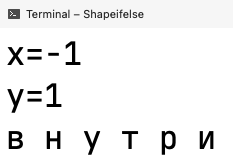
\includegraphics[width=0.3\textwidth]{images/task-1-1.png}
    \caption{Ввод координат внутри области}
    \label{fig:task-1-1}
\end{figure}

\begin{figure}[H]
    \centering
    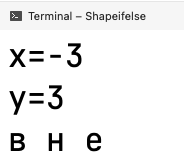
\includegraphics[width=0.3\textwidth]{images/task-1-2.png}
    \caption{Ввод координат вне области}
    \label{fig:task-1-2}
\end{figure}

\begin{figure}[H]
    \centering
    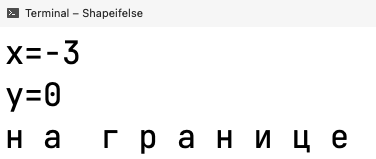
\includegraphics[width=0.3\textwidth]{images/task-1-3.png}
    \caption{Ввод координат на границе области}
    \label{fig:task-1-3}
\end{figure}

\subsection{Применение оператора switch}

Проделав все шаги из задания, я получил следующий исходный код:
\inputminted{csharp}{../Calc_switch/Calc_switch/Program.cs}

На рис. \ref{fig:task-2-1} представлена работа приложения с корректными данными.

\begin{figure}[H]
    \centering
    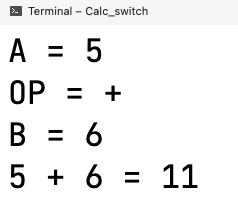
\includegraphics[width=0.3\textwidth]{images/task-2-1.png}
    \caption{Работа приложения с корректными данными}
    \label{fig:task-2-1}
\end{figure}

На рис. \ref{fig:task-2-2} показан случай деления числа на ноль. В результате работы программы мы получили бесконечность. Это связано с тем, что при делении числа с плавающей запятой на ноль по стандарту IEEE 754 должно получится число, представляющее бесконечность.

\begin{figure}[H]
    \centering
    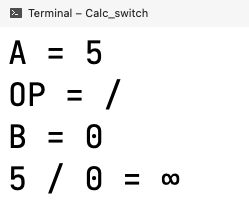
\includegraphics[width=0.3\textwidth]{images/task-2-2.png}
    \caption{Деление числа на ноль}
    \label{fig:task-2-2}
\end{figure}

На рис. \ref{fig:task-2-3} показан случай деления нуля на ноль. Также, как и предыдущем случае, стандарт IEEE 754 указывает, что при делении нуля на ноль (т. е. при любой математически неопределенной операции) результатом должен быть NaN (not a number).

\begin{figure}[H]
    \centering
    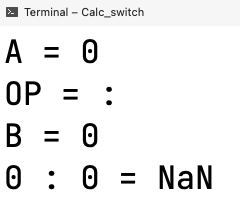
\includegraphics[width=0.3\textwidth]{images/task-2-3.png}
    \caption{Деление нуля на ноль}
    \label{fig:task-2-3}
\end{figure}

На рис. \ref{fig:task-2-4} представлен случай использования неправильного символа операции. В данном случае программа отработала корректно и сообщила об этом пользователю.

\begin{figure}[H]
    \centering
    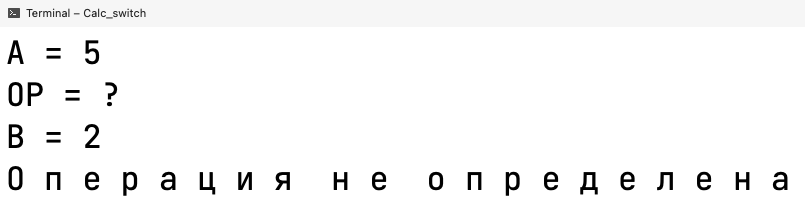
\includegraphics[width=0.5\textwidth]{images/task-2-4.png}
    \caption{Использование неизвестного оператора}
    \label{fig:task-2-4}
\end{figure}

\subsection{Определение високосного года}

В своей программе я считываю год со стандартного ввода, а затем проверяю, кратен ли год 4 и при этом не кратен 100, или же кратен ли он 400. Если одно из этих условий выполняется, я выводу YES, а иначе -- NO. Исходный код программы представлен в следующем листинге:
\inputminted{csharp}{../LeapYear/LeapYear/Program.cs}

На рис. \ref{fig:task-3-1}, \ref{fig:task-3-2} и \ref{fig:task-3-3} я проверяю работу программы для разных годов с разной кратностью.

\begin{figure}[H]
    \centering
    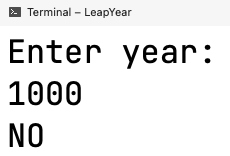
\includegraphics[width=0.3\textwidth]{images/task-3-1.png}
    \caption{Год кратный 4 и кратный 100}
    \label{fig:task-3-1}
\end{figure}

\begin{figure}[H]
    \centering
    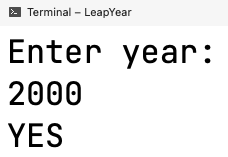
\includegraphics[width=0.3\textwidth]{images/task-3-2.png}
    \caption{Год кратный 4, кратный 100 и кратный 400}
    \label{fig:task-3-2}
\end{figure}

\begin{figure}[H]
    \centering
    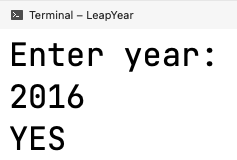
\includegraphics[width=0.3\textwidth]{images/task-3-3.png}
    \caption{Год кратный 4}
    \label{fig:task-3-3}
\end{figure}

\section{Реализация циклов при работе с данными размерных типов}

\subsection{Использование операторов цикла while, do while и for}

Я выполнил все шаги из задания и получил следующий исходный код:

\inputminted{csharp}{../Loop/Loop/Program.cs}

Результат работы программы показан на рис. \ref{fig:task-4-1}.

\begin{figure}[H]
    \centering
    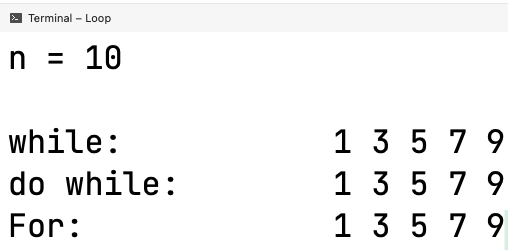
\includegraphics[width=0.4\textwidth]{images/task-4-1.png}
    \caption{Результат работы программы}
    \label{fig:task-4-1}
\end{figure}

После этого я реализовал следующую программу, использующую цикл с постусловием. Эта программа принимает на вход левую и правую границу интервала, после чего выводит значение синуса для каждого \(x\) с шагом \(0.01\). Исходный код программы представлен в следующем листинге:

\inputminted{csharp}{../Loop/Loop/Program1.cs}

На рис. \ref{fig:task-4-2} представлен результат работы программы.

\begin{figure}[H]
    \centering
    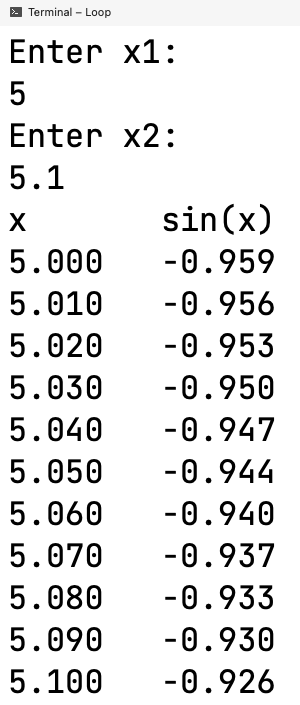
\includegraphics[width=0.3\textwidth]{images/task-4-2.png}
    \caption{Результат работы программы}
    \label{fig:task-4-2}
\end{figure}

Затем я выполнил следующие задание и реализовал программу с циклом с предусловием. В этой программе используется алгоритм Евклида для поиска НОД. Ее исходный код представлен в следующем листинге:

\inputminted{csharp}{../Loop/Loop/Program2.cs}

На рис. \ref{fig:task-4-3} представлен результат работы программы.

\begin{figure}[H]
    \centering
    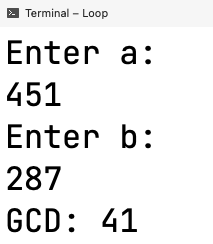
\includegraphics[width=0.3\textwidth]{images/task-4-3.png}
    \caption{Результат работы программы}
    \label{fig:task-4-3}
\end{figure}

После этого задачу вывода значений функции с помощью цикла с предусловием. Единственное изменение, которое необходимо внести, чтобы программы остались эквивалентными -- проверка на равенство текущего значения \texttt{x} и значения \texttt{x1}. Если этого не сделать, то в случае, когда \texttt{x > x2}, цикл не будет выполнен ни разу. Исходный код решения представлен в следующем листинге:

\inputminted{csharp}{../Loop/Loop/Program4.cs}

Затем я реализовал алгоритм Евклида с помощью цикла с постусловием. Кроме изменения самого цикла, пришлось добавить проверку на неравенство аргументов \texttt{a} и \texttt{b}. Это необходимо, поскольку иначе, если на вход будут переданы равные значения \texttt{a} и \texttt{b}, программа попадет в бесконечный цикл. Исходный код программы представлен в следующем листинге:

\inputminted{csharp}{../Loop/Loop/Program3.cs}

\subsection{Расчет суммы, используя операторы перехода}


Выполнив все шаги из задания, я получил следующий исходный код:

\inputminted{csharp}{../Sum/Sum/Program.cs}

На рис. \ref{fig:task-5} показан пример работы программы.

\begin{figure}[H]
    \centering
    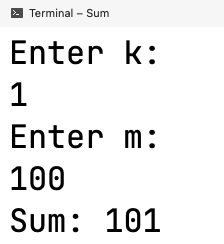
\includegraphics[width=0.3\textwidth]{images/task-5.png}
    \caption{Пример работы программы Sum}
    \label{fig:task-5}
\end{figure}

\subsection{Стрельба по мишени}

Моя программа разработана для второго варианта. В своей программе я сначала генерирую случайные значения координат мишени. После этого запускаю цикл из трех выстрелов. При каждом выстреле я считываю значения координат от пользователя. Если пользователю не повезло и ему помешали, его значения координат заменяются на случайные. После этого я рассчитываю расстояние до центра мишени. В зависимости от того, в какое место попал пользователь, начисляется разное количество очков. После каждого выстрела пользователю сообщается текущее количество очков. Исходный код программы представлен в следующем листинге:

\inputminted{csharp}{../TargetShooting/TargetShooting/Program.cs}

На рис. \ref{fig:task-6} показан пример работы программы.

\begin{figure}[H]
    \centering
    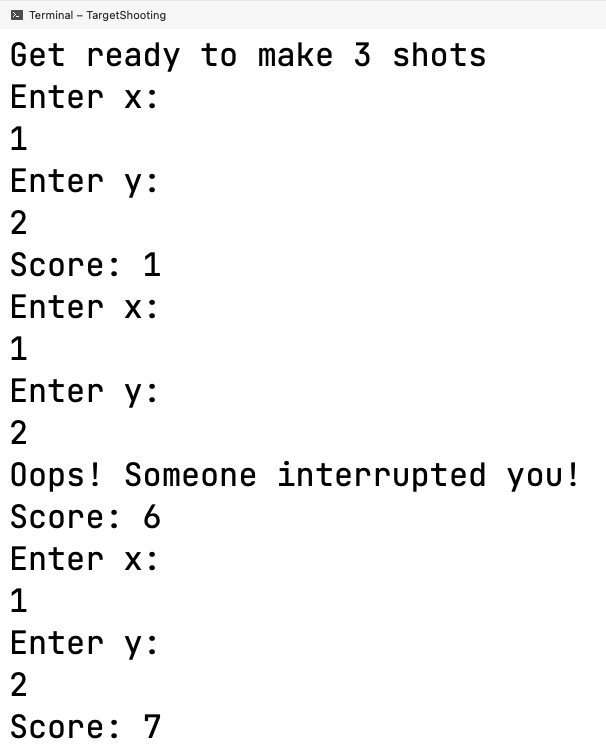
\includegraphics[width=0.4\textwidth]{images/task-6.png}
    \caption{Пример работы программы}
    \label{fig:task-6}
\end{figure}

\end{document}
